\chapter{Introducing directionality with diffusion tensors}
\label{chap:dti}
\index{DTI} In this chapter, we focus on how to transfer information
from diffusion tensor imaging (DTI) data to our finite element
methods. To do so, we will need to overcome a few practical
challenges. In particular, the raw DTI data can contain
non-physiological data, especially near the CSF. Moreover, the raw DTI
data is represented both in terms of a different coordinate system and
at a different resolution than the computational mesh. To overcome the
first challenge, we will use local extrapolation of nearby valid
values; to overcome the second challenge, we will
co-register\footnote{See Section~\ref{sec:chp-dti:freesurfer-coord}.}
the data with the images used to construct the computational mesh.

Concretely, we will
\begin{itemize}
\item
  Process the diffusion tensor images to extract mean diffusivity and
  fractional anisotropy\footnote{Mean diffusivity and fractional 
  anisotropy are defined in~\eqref{eqn:chp5:md} and 
  \eqref{eqn:chp5:fa}, respectively.} data, and
\item
  Map the DTI tensor data into a finite element representation created from
  the T1-weighted images.
\end{itemize}

\section{Extracting mean diffusivity and fractional anisotropy}

\subsection{Extracting and converting DTI data}
\label{sec:chp-dti:extract-and-convert}
\index{DicomBrowser}
\index{FreeSurfer!\emp{mri\_convert}}
The DTI data must first be extracted from a DICOM dataset. We use
DicomBrowser to extract a DTI series from the book data-set in
Chapter~\ref{sec:chp2:tools:viewers}, and the resulting files are
available in \emp{dicom/ernie/DTI}. Our next task is to convert the
extracted DTI images to a single volume image and to produce
supplementary information files about the DTI image data for
downstream postprocessing.  Various open source tools are available
for the processing of DTI data \cite{soares2013hitchhiker}. Here, we
continue to use \freesurfer{} and its associated command-line tools. 
As in chapter~\ref{sec:chp3:surfaces}, we can select any of the files 
extracted from the \emp{DICOM} DTI data (\emp{dicom/ernie/DTI}) to start 
the process; here, we arbitrarily choose \emp{IM\_1496} and launch the 
{\freesurfer} command \emp{mri\_convert}:
\terminal{\$ cd dicom/ernie/DTI \\
\$ mri\_convert IM\_1496 dti.mgz
}

This process, when successful, creates three files: \emp{dti.mgz},
\emp{dti.bvals}, and \emp{dti.voxel\_space.bvec}.  The last two, plain
text files, contain information regarding the b-values and
b-vectors associated with the DTI data.  %These vectors and values indicate 
%the direction in which the diffusion weighting is applied (b-vectors) and 
%the magnitude of the value (b-values) of that weighting. 
% 
%These values and vectors
%measure the degree of the diffusion weighting applied in the imaging
%process (b-values) and in what direction (b-vectors). 
%The various slices in the imaging sequence are measured for the different 
%b-values and b-vectors selected for the initial imaging study (see
%Figure~\ref{fig:chp5:DTIslices}).
The b-vectors and b-values are selected as part of the imaging process; they 
determine the direction (b-vector) and strength (b-value) of the pulsed  
magnetic diffusion gradient used during the diffusion weighted imaging scan.  
For instance, Figure~\ref{fig:chp5:DTIslices} shows an axial slice measured 
with the same choice of b-value but different b-vectors.  Once the scan has 
taken place, we can read this information but it cannot be altered without 
scanning the patient again.  
\begin{figure}	
\begin{center}
  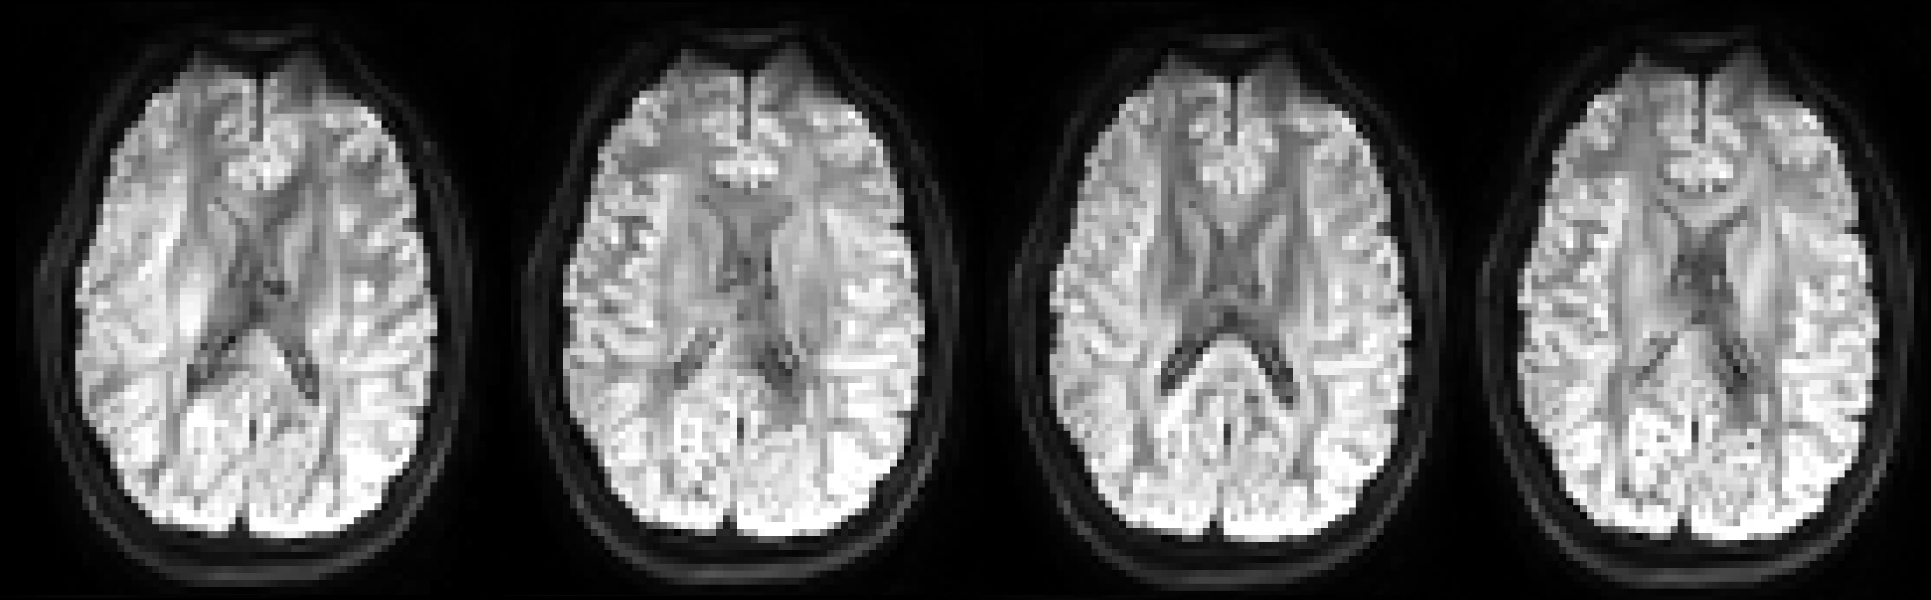
\includegraphics[width=0.95\textwidth]{./graphics/chp5/dwi.png}
\end{center}
\caption{Axial DTI slices measured with different b-vectors. The
  resolution in the diffusion tensor image is typically lower (here, 96x96x50)
	compared to that in the T1 images; the latter are, canonically, 
	256x256x256.}
\label{fig:chp5:DTIslices}
\end{figure}

\subsection{DTI reconstruction with \freesurfer}
\label{sec:chp-dti:freesurfer-dtrecon}
\index{FreeSurfer!\emp{dt\_recon}}
Next, we aim to reconstruct comprehensive DTI data from the volume,
b-value, and b-vector files using the \freesurfer{} command
\emp{dt\_recon}. The command takes an input volume (following
\emp{-{}-i}), b-vector and b-values files (following \emp{-{}-b}), an
output directory \emp{-{}-o}, and the \emp{recon-all} subject ID
\emp{-{}-s} (see Chapter~\ref{sec:chp3:surfaces}). Within our book data 
directory \emp{dicom/ernie/DTI}, we can launch the following commands:
\terminal{\$ export SUBJECTS\_DIR=my-freesurfer-dir \\
  \$ dt\_recon -{}-i dti.mgz -{}-b dti.bvals dti.voxel\_space.bvecs -{}-s ernie -{}-o \$SUBJECTS\_DIR/ernie/dti}
\noindent with \emp{my-freesurfer-dir} replaced by the FreeSurfer subject's
directory (e.g. \emp{freesurfer/} from the book data-set).

\index{FreeSurfer!\emp{bbregister}}
This command produces multiple output files\footnote{The command above will 
store the files in \$SUBJECTS\_DIR/ernie/dti.  Alternatively, you can run 
\emp{mri2fem/chp5/all.sh} which will create a directory 
\emp{mri2fem/chp5/ernie-dti} that includes the same set of the files as well. 
You will need FSL installed to use \emp{dt\_recon} (see 
Chapter~\ref{sec:chp2:tools:freesurfer}).}, including
\emp{tensor.nii.gz}, \emp{register.dat}, and \emp{register.lta}. The
registration in \emp{dt\_recon} uses the registration command
\emp{bbregister}\footnote{This registration step is done automatically by 
{\freesurfer} using the subject's previously {\freesurfer}-processed data that 
is assumed to be available at this stage of the book; see 
Chapter~\ref{sec:chp3:surfaces} for the necessary steps. The mathematical 
details of co-registration are further discussed in 
Section~\ref{sec:chp-dti:freesurfer-coord}.} to register the DTI
data~\cite{freesurfer-wiki}. Files with the suffix .nii are in the
NIfTI format. Of these, \emp{tensor.nii.gz} is the spatially varying
diffusion tensor. Further, an eigendecomposition of this tensor in
terms of spatially varying eigenvalues $\lambda_1$, $\lambda_2$, and 
$\lambda_3$ and eigenvectors $v_1$, $v_2$, and $v_3$ is given in the files
\emp{eigvals.nii.gz} and \emp{eigvec1.nii.gz},\emp{eigvec2.nii.gz},
and \emp{eigvec3.nii.gz}.


\subsection{Mean diffusivity and fractional anisotropy}
\index{mean diffusivity}
\index{fractional anisotropy}
In addition, \emp{dt\_recon} produces the NIfTI files
\emp{adc.nii.gz} and \emp{fa.nii.gz} for the mean (or apparent)
diffusivity (MD) and fractional anisotropy (FA), respectively. 
The mean diffusivity is given by 
\begin{equation}\label{eqn:chp5:md}
  \rm{MD} = \frac{1}{3}(\lambda_1 + \lambda_2 + \lambda_3),   
\end{equation}
and  fractional
anisotropy is defined~\cite{kindlmann2007geodesic} by
\begin{equation}\label{eqn:chp5:fa}
	\rm{FA}^2 = \frac{1}{2} \frac{(\lambda_1-\lambda_2)^2 
+ (\lambda_2 - \lambda_3)^2 + (\lambda_3 - \lambda_1)^2}{\lambda_1^2 
+ \lambda_2^2 + \lambda_3^2} .  
\end{equation}
\index{file format!NIfTI}
\begin{figure}	
  \begin{center}
    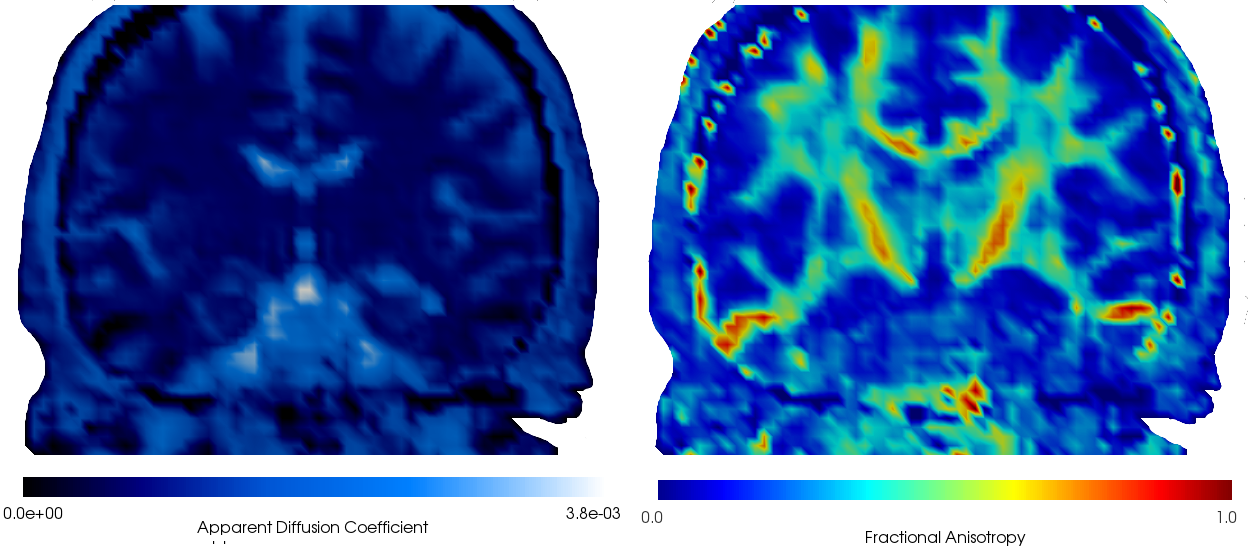
\includegraphics[width=0.95\textwidth]{./graphics/chp5/paraview_adcfa.png}
  \end{center}
  \caption{Mean diffusivity (left) and fractional anisotropy (right) as shown in \emp{ParaView}.}
  \label{fig:chp5:DTIfa}
\end{figure}
NIfTI files can be viewed in ParaView. You might first need to enable
the NIfTI viewer plugin by selecting the ParaView menu option labeled
\button{Tools$\rightarrow$Manage Plugins}, selecting the plugin option%
\footnote{The correct plugin may also be named AnalyzeNifTIIO in earlier 
versions (i.e.~before 5.7.0) of ParaView.} 
\button{AnalyzeNifTIReaderWriter} and then clicking \button{Load Selected}. You
can then open and view .nii files in ParaView, just as you would any other
file. To unzip .nii.gz to .nii, one can use \emp{mri\_convert}:
\terminal{\$ mri\_convert adc.nii.gz adc.nii \\ 
\$ mri\_convert fa.nii.gz fa.nii} 

\noindent Lets open \emp{adc.nii} and verify that we can reproduce 
Figure~\ref{fig:chp5:DTIfa} (left); the process will be the same for 
\emp{fa.nii}.  After loading the AnalyzeNifTIIO plugin, described above, 
and opening \emp{adc.nii} click \button{Apply}.  You will likely see an 
empty three-dimensional cube in the view window.  In the left pane, 
find the \emp{Representation} option and change this to \emp{Volume}.  You 
should now see something that looks similar to a `brain in a box' viewed from 
the top. Now click \button{Filters$\rightarrow$Alphabetical} and select 
\emp{Slice}.  In the left pane, find the option labeled \emp{Normal}; it 
should be under the option labeled \emp{Origin}.  Change the \emp{Normal} 
from \emp{1 0 0} to \emp{0 1 0} and click \button{Apply}.  

In the left pane, once more, hide the object \emp{adc.nii} by clicking the 
picture of the eye next to its name.  Now, rotate the view window so that you 
can see the X-Z plane; the result should look similar to 
Figure~\ref{fig:chp5:DTIfa}.  We can make it look more similar by changing the 
color scheme.  In the left pane, find the section labeled \emp{Coloring}.  Mouse 
over the buttons here until you find the button labeled \emp{Choose preset}. 
Click this and select the \emp{Black, blue and white} color scheme, 
click \button{Apply} and then close the color scheme preset window.  The image 
you see now was saved and post-processed to remove the border outside the 
skull to produce Figure~\ref{fig:chp5:DTIfa} (left).  You can repeat these 
steps with \emp{fa.nii}, this time using the \emp{jet} color scheme, to 
reproduce Figure~\ref{fig:chp5:DTIfa} (right).

Generally, the average FA value is around 0.5 and changes by around 2\%
during day/night~\cite{voldsbekk2020evidence}.  Anisotropy decreases
with age, for example, around 14\% from 30 to 80
years~\cite{kochunov2011fractional} and can change by up to
50\% in certain areas of an Alzheimer's disease patient compared with
healthy subjects~\cite{naggara2006diffusion}. In the \emp{ernie} data 
(Figure~\ref{fig:chp5:DTIfa}), the median white matter FA value is
0.3, with a minimum of 0.009 and a maximum of 0.9998.

\section{Finite element representation of the diffusion tensor}

In this section, we aim to
\begin{itemize}
\item
  Ensure that the DTI data have a valid eigendecomposition (with positive eigenvalues),
\item
  Map the DTI tensor into a finite element tensor function defined on
  a finite element mesh, and
\item
  Briefly discuss co-registration.
\end{itemize}

\subsection{Preprocessing the diffusion tensor data}
\index{preprocessing DTI data}

The DTI data can be quite rough compared to the T1 data and our
corresponding finite element meshes; DTI data is typically at a low resolution 
of 96x96x50 while T1 resolution is typically much higher at 
256x256x256\footnote{See Figure~\ref{fig:chp2:t1vt2} (left) versus 
Figure~\ref{fig:chp5:DTIslices}.}. Moreover, the signal can be disturbed near 
the cerebrospinal fluid (CSF), which makes the data in certain areas of the 
cortical grey matter and in regions near the ventricle system less reliable. 
Indeed, inspection of the eigenvalues of the DTI tensor shows 
non-physiological (zero and/or negative) eigenvalues. To ensure a 
physiologically (and mathematically) reasonable diffusion tensor, we recommend 
preprocessing the diffusion tensor prior to numerical simulation. In 
particular, we present in this chapter two scripts that
\begin{itemize}
\item
  Check the DTI tensor data for non-physiological values and
\item
  Replace non-physiological with physiological values in the DTI tensor,
\end{itemize}
respectively.

\subsubsection*{Creating brain masks}
\index{FreeSurfer!\emp{mri\_binarize}}
First, we will use \freesurfer{} to create so-called
masks of the brain. A mask is a type of filter where voxels (significantly) 
outside the brain are set to zero and all other voxels are set to a value of one.  
Using our white matter parcellation data (included in 
\emp{freesurfer/ernie/mri/wmparc.mgz}), we can create brain masks as follows:
\terminal{\$ mri\_binarize --i wmparc.mgz --gm --dilate 2 --o mask.mgz}
\noindent The \emp{dilate} flag determines the extent to which the mask should be extended 
outside the brain surface provided by
\emp{wmparc.mgz}. Examples of such masks are shown in
Figure~\ref{fig:chp5:masks}.
\begin{figure}	
\begin{center}
  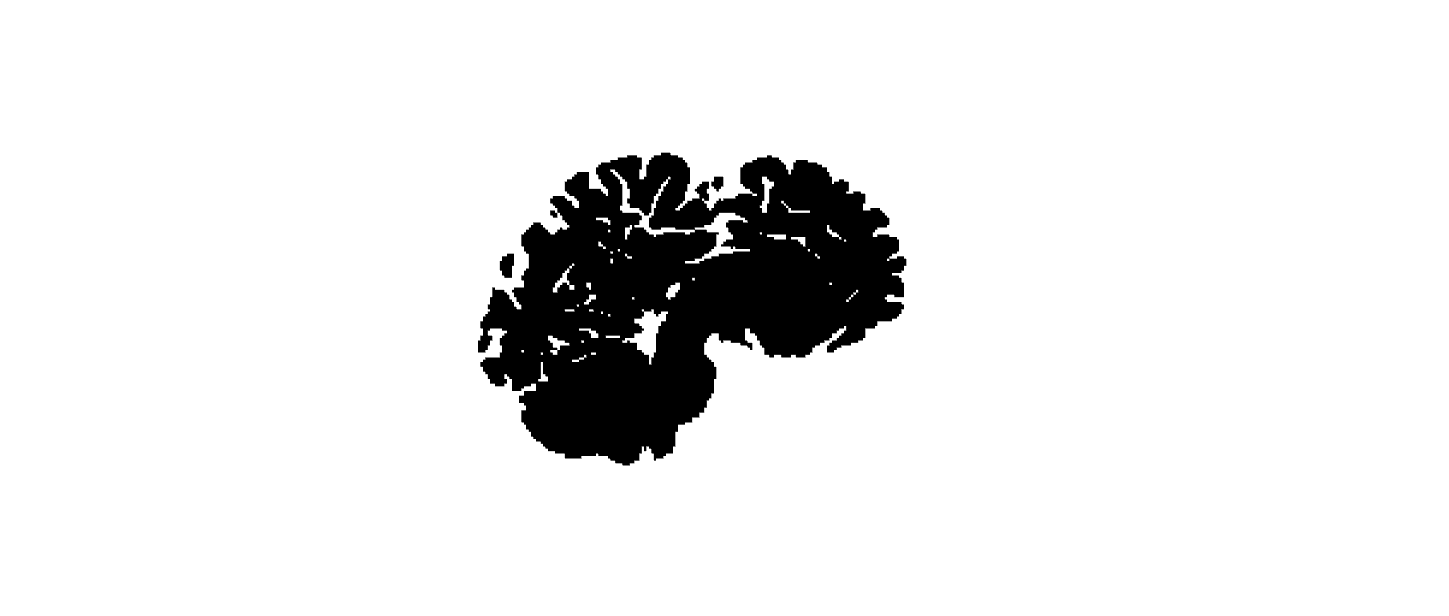
\includegraphics[trim=400 130 500 150,clip,width=0.49\textwidth]{./graphics/chp5/mask0.png}
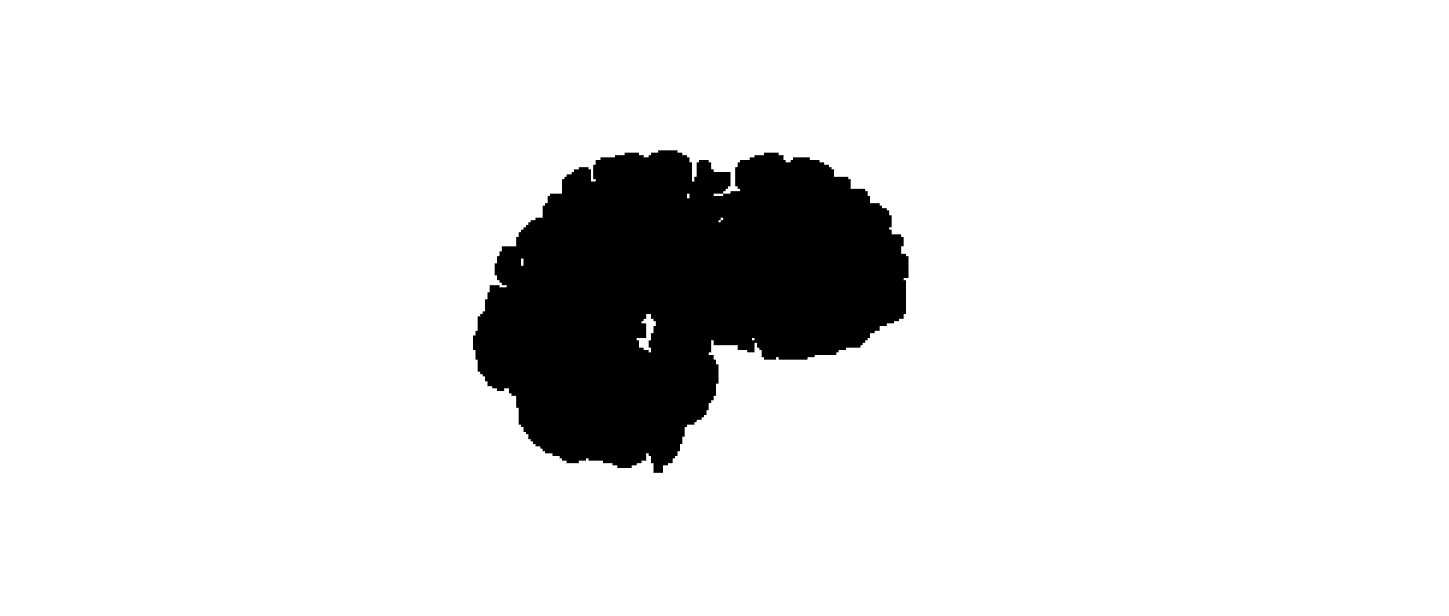
\includegraphics[trim=400 130 500 150,clip,width=0.49\textwidth]{./graphics/chp5/mask1.png} \\
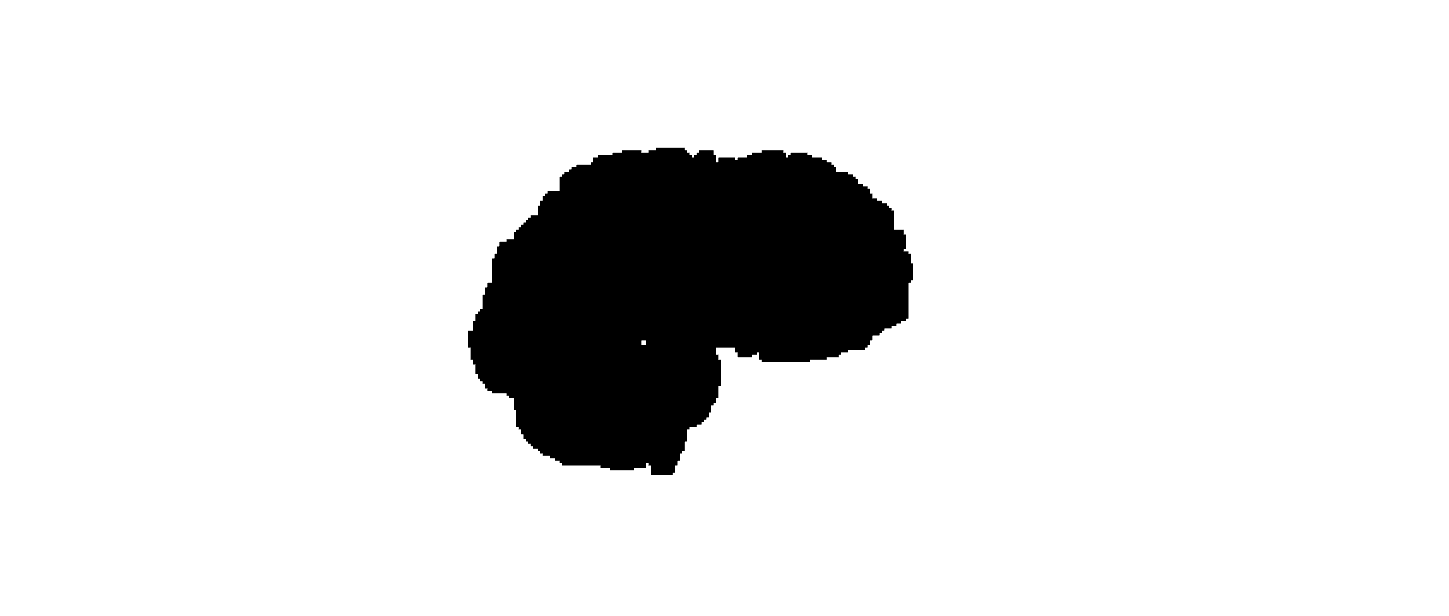
\includegraphics[trim=400 130 500 150,clip,width=0.49\textwidth]{./graphics/chp5/mask2.png}
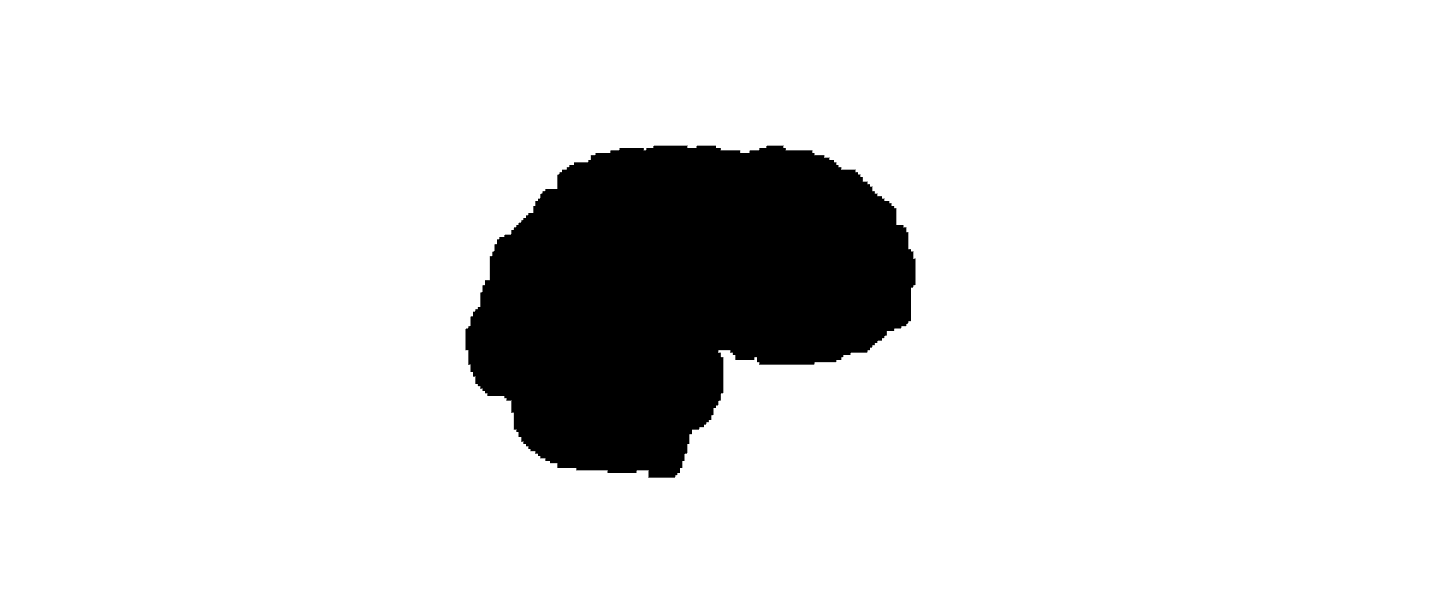
\includegraphics[trim=400 130 500 150,clip,width=0.49\textwidth]{./graphics/chp5/mask3.png}
\end{center}
\caption{
  Brain masks created using \emp{mri\_binarize} with \emp{dilate} ranging from zero to three.
}
\label{fig:chp5:masks}
\end{figure}

\subsubsection*{Examining the DTI data values}
\index{voxel space}
We can work with the DTI data in a very similar manner as we did
for the parcellation (image) data in
Chapter~\ref{sec:chp4:mapping_parcellation}. We will again use NiBabel
to load the image data, use the \emp{vox2ras} functions for the mapping
between the different image coordinate systems (DTI voxel space and T1
voxel space), and process the data as NumPy arrays. The complete
script can be run as
\terminal{\$ cd mri2fem/chp5\\
\$ python3 check\_dti.py -{}-dti tensor.nii.gz -{}-mask mask.mgz}

We import the key packages:
\newpythonsnippet{chp5}{check_dti.py}{1}{6}

\noindent We define the function \emp{check\_dti\_data} that takes the DTI
tensor and mask files as input: 
\newpythonsnippet{chp5}{check_dti.py}{8}{20}

\noindent Now, the important coordinate transformations can be handled as follows:
\newpythonsnippet{chp5}{check_dti.py}{21}{30}

\noindent Before computing eigenvalues, we run
\newpythonsnippet{chp5}{check_dti.py}{33}{37}
and we compute the fractional anisotropy and check the validity of each voxel value, as follows:
\newpythonsnippet{chp5}{check_dti.py}{46}{63}
The above snippet makes use of the function \emp{compute\_FA}, which is also 
defined in \emp{check\_dti.py}, to compute \eqref{eqn:chp5:fa}.  The result is 
a vector \emp{FA} whose entries contain the fractional anisotropy computed at 
each available DTI data location. The term \emp{positives} is a binary vector, with the 
same number of entries as \emp{FA}; it has a value of one if all three of the eigenvalues 
for the region corresponding to the array index are positive, and zero otherwise. 
The vector \emp{valid} is therefore a second binary vector whose indices correspond 
to the locations where DTI data are available.  The value at each index of \emp{valid} 
is one precisely when all of the eigenvalues are positive and the fractional anisotropy 
there is larger than zero but less than one.  The \emp{valid} vector is therefore 
a mask that indicates where the DTI tensor contains physically admissible values.
The \emp{valid} mask is then reshaped\footnote{The term \textit{reshaped} here 
means that the (tensor) data is re-organized into an expected form. An example 
would be reshaping a $1\times 9$ (row) tensor to a $3\times 3$ (matrix) tensor 
by putting the first three entries, of the $1\times 9$ tensor, in the first 
row, the next three in the second row and the last three in the final row of 
the $3\times 3$ tensor.} 
to fit the dimensions of the original \emp{mask}, created from the 
\emp{mask\_file}, and the number of zeros, corresponding to invalid entries, is 
computed and reported in the final lines.

\subsubsection*{Improving DTI values by extrapolation and resampling to T1 space}
If numerous invalid DTI voxel data are reported, by \emp{check\_dti.py} as 
discussed above, we can attempt to improve the DTI data by extrapolating from 
adjacent valid voxel locations to correct nearby invalid data.  The 
correction script is \emp{mri2fem/chp5/clean\_dti\_data.py} and can be run as
\terminal{\$ cd mri2fem/chp5\\
%\$ python3 clean\_dti\_data.py -{}-dti tensor.nii.gz -{}-mask mask.mgz -{}-out\_nii tensor-clean.nii}
\$ python3 clean\_dti\_data.py -{}-dti tensor.nii.gz -{}-mask mask.mgz -{}-out tensor-clean.nii}
\noindent and the main functionality reads 
\newpythonsnippet{chp5}{clean_dti_data.py}{26}{48}

The first operation carried out by the \pythoninline{clean\_dti\_data} function 
is to call \pythoninline{check\_dti\_data}, which we discussed in the previous 
section.  Recall that, among other things, the \pythoninline{check\_dti\_data} 
function returns a tensor representation (\emp{D}) of the DTI data that has been 
converted from DTI voxel space coordinates to T1 voxel space coordinates%
\footnote{T1 coordinates are the same coordinates used by the computational 
meshes that were constructed, in previous chapters, from the surfaces extracted 
from {\freesurfer} segmented T1 data.  Thus, \emp{D} is now expressed in terms 
of coordinates that make sense when used alongside the computational meshes}.
Next, we will first search for a valid tensor in directly adjacent voxels;
this is done using the function \pythoninline{find_valid_adjacent_tensor} 
defined in \emp{clean\_dti\_data.py}. If no valid tensor is found nearby, the 
search range is iteratively increased.  %
%
%Next, the function \pythoninline{find_valid_adjacent_tensor}, defined in 
%\emp{clean\_dti\_data.py}, will first search for a valid
%tensor in directly adjacent voxels; if no valid tensor is found nearby, the 
%search range is iteratively increased.  
The script determines that a nearby tensor, in the valid region, contains valid 
data if a non zero mean diffusivity (MD) is also calculated there.  Once one, 
or more, nearby valid value(s) are found, replacement data is chosen.  If only 
one valid value is found, it is directly used.  If there are multiple valid 
tensors within the search range, the tensor data\footnote{Due to the way in 
which the \emp{valid} mask is constructed, a tensor with invalid data can 
violate either the required condition that all of the eigenvalues must 
satisfy $\lambda_i > 0$ or the required condition that the FA must 
satisfy $0<$FA$<1$.  In either case, the search for a nearby valid tensor 
identifies a nearby candidate and replaces the whole of the tensor information 
at the invalid tensor location.  Thus, all of required conditions are satisfied, 
at the previously invalid location, after the data replacement.} with MD value 
closest to the median of the non-zero MD is chosen as a replacement: 
\newpythonsnippet{chp5}{clean_dti_data.py}{7}{24}

\subsection{Representing the DTI tensor in \fenics{}}
\label{chp5:sec:loading-dti-tensor}
\index{DTI}
\index{FEniCS!\emp{TensorFunctionSpace}}

With the DTI data checked and potentially improved, we are now ready to map 
our preprocessed DTI image (now in T1 voxel space) onto a FEniCS mesh.  We will 
use the code located in \emp{mri2fem/chp5/dti\_data\_to\_mesh.py} to accomplish this 
task. To begin, we assume that we have a \emp{mesh} available (e.g.~%
\emp{ernie-brain-32.h5} from Chapter~\ref{chp4:meshio-converting}), that we have 
loaded the clean DTI image and data in \emp{dti\_image} and \emp{dti\_data}, respectively, 
and that we have the \emp{ras2vox} transform associated with this image.  We can retrieve 
the \emp{vox2ras} and \emp{ras2vox} transformations associated with the data 
by 
\newpythonsnippet{chp5}{dti_data_to_mesh.py}{49}{51}

To represent the diffusion tensor in FEniCS, we create a FEniCS
\emp{Function} over a \emp{TensorFunctionSpace} of (discontinuous)
piecewise constant polynomial fields (\emp{"DG", 0}): 
\newpythonsnippet{chp5}{dti_data_to_mesh.py}{53}{55}

For each cell, we need to associate an identifying coordinate value so
that we can associate the cells of our mesh to the voxel data.  One
possibility is to extract the cell midpoints as we have done before;
here, we opt to extract the coordinates of the degrees of
freedom associated with a DG \emp{FunctionSpace} object that we will 
define on our mesh and convert these to voxel indices:
\newpythonsnippet{chp5}{dti_data_to_mesh.py}{57}{68}

\noindent The above snippet first retrieves the coordinates of the
\emp{TensorFunctionSpace} degrees of freedom on our mesh and applies
the \emp{ras2vox} transformation to determine coordinates in voxel
space.

We can now reshape the DTI data into a cell-wise structure based on
the extracted indices\footnote{Voxels are located based on the degree
  of freedom (DOF) coordinates from the \emp{FunctionSpace} object. This
  approach guarantees that there are no missing values as every coordinate
  maps to some voxel. However, some voxels may correspond to more
  than one mesh cell as there may be more cells in the mesh than there
  are voxels e.g.~if the mesh has a resolution which is less than the 
  resolution of the T1 (voxel) image space.} (now in voxel space):
\newpythonsnippet{chp5}{dti_data_to_mesh.py}{70}{72}
\noindent With the reshaped DTI data in hand, we assign these to a {\fenics} tensor 
field, \pythoninline{D}, allowing the data to be saved alongside the mesh data.
\index{fractional anisotropy}
\newpythonsnippet{chp5}{dti_data_to_mesh.py}{78}{79}
The {\fenics} tensor field DTI data can be saved alongside the mesh for later use 
in {\fenics} simulations with 
\newpythonsnippet{chp5}{dti_data_to_mesh.py}{87}{90}
The resulting fiber directions, shown in Figure~\ref{fig:chp5:freesurfer-parc}, 
can be inspected visually.
\begin{figure}	
  \begin{center}
  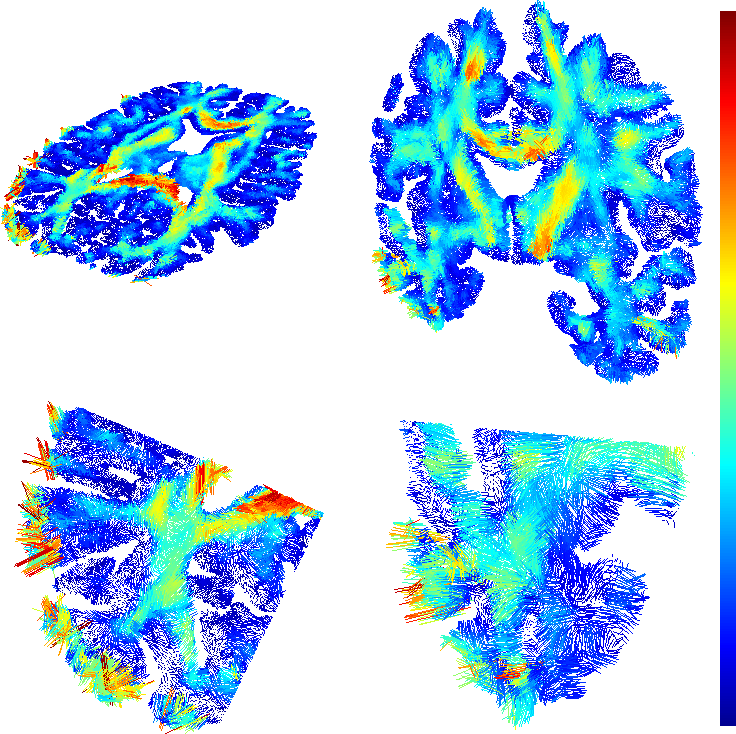
\includegraphics[width=0.8\textwidth]{./graphics/chp5/fiber-fa-2cb.png}
  \end{center}
\caption{Upper panels show fiber directions (DTI eigenvectors) colored
  by the fractional anisotropy in the axial and coronal planes. The lower 
  panels show a zoom focusing on the boundary between grey matter and the 
  cerebrospinal fluid. Note that the vector nature of the data can be seen 
  more clearly in bottom panel images where the fibers can be seen to have 
  clear directionality.}
\label{fig:chp5:freesurfer-parc} 
\end{figure}

\subsection{A note on co-registering DTI and T1 data}
\label{sec:chp-dti:freesurfer-coord}
\index{co-registration}
As we have seen, {\freesurfer} uses several different coordinate
systems to label the position of data in its various output files.
Thus, to combine different types of data into something we can use in
{\fenics} simulations, we need to extract information about the
different coordinate systems used in the files and be able to map
between these different coordinate systems. This process is known as
co-registration. The scripts we have presented use NiBabel
functionality to handle co-registration; this section provides 
additional information regarding co-registration, for both context and
completeness.

In short, let $x_1 = (x_1, y_1, z_1)$ and $x_2 = (x_2, y_2, z_2)$ represent the
same physiological point in $\R^3$ but represented with respect to two
different coordinate systems (bases). Then, there is an affine
transformation such that
\begin{equation}\label{eqn:chp5:affinet}
x_2 = A\, x_1 + b,
\end{equation}
for $A \in \R^{3 \times 3}$ and $b \in \R^3$. The mapping is often
stored instead as a $4\times4$ matrix, where the last row can be
ignored.  As this equivalent $4\times 4$ representation often appears in the 
discussions, and software documentation, within the neuroimaging community, 
we also show it here; the above affine transformation \eqref{eqn:chp5:affinet} 
can also be written as 
\begin{equation*}
\left[\begin{array}{c}
x_{2}\\
y_{2}\\
z_{2}\\
1
\end{array}\right] = 
\left[
\begin{array}{cccc}
a_{11} & a_{12} & a_{13} & b_1 \\
a_{21} & a_{22} & a_{23} & b_2 \\
a_{31} & a_{32} & a_{33} & b_3 \\
0      &    0   &   0    & 1
\end{array}
\right]
\left[
\begin{array}{c}
x_1\\
y_1\\
z_1\\
1
\end{array}
\right],
\end{equation*}
where the $a_{ij}$ are the entries of the matrix $A$ and the $b_i$ are the 
entries of the vector $b$. 


The term \textit{co-registration} specifically refers to the
determination of the transformation matrix $A$ and vector $b$
corresponding to a pair of files.  %
%
\index{FreeSurfer!\emp{mri\_info}}
A key step in the co-registration of T1 and DTI images, or any pair
of images in general, is to ascertain the type of coordinate system
used when initially storing these images. Towards this end, we can
make use of the \emp{mri\_info} command.  Coordinate system
information regarding the {\freesurfer}-processed T1 images is stored
in the file \emp{orig.mgz}. We can interrogate this file by:
\terminal{\$ cd \$SUBJECTS\_DIR/ernie/mri \\
\$ mri\_info orig.mgz -{}-orientation \\
LIA}

\noindent The output \emp{LIA} means that the T1 image files were
generated with respect to the `Left Inferior Anterior' coordinate
system (see~\cite{freesurfer-wiki} for details).  Coordinate system
information regarding the {\freesurfer}-processed DTI images is stored
in the file \emp{tensor.nii.gz}. We can interrogate this file, once
more using \emp{mri\_info}, by:

\terminal{\$ cd \$SUBJECTS\_DIR/ernie/dti \\
\$ mri\_info tensor.nii.mgz -{}-orientation \\
LPS}

The coordinate systems can be understood as follows: the positive
direction in the sagittal plane can be either (L)eft or (R)ight, the
positive direction in the coronal plane can be either (P)osterior or
(A)nterior, and the positive direction in the axial plane can be either
(I)nferior or (S)uperior. Furthermore, the order of the planes can be
different, that is, the third axis might not correspond to the axial
plane. For instance, let us examine the coordinate systems described
by the abbreviations \emph{LIA} and \emph{LPS}. We see that the coronal
plane corresponds to the third axes (A) in \emph{LIA} and second axes
(P) in \emph{LPS}, and we have the opposite for the axial plane (I
vs.~S). Thus, these coordinates systems differ by the choice of a 
positive direction in the coronal and axial planes, in addition to
their order.

Both coordinates systems describe voxel spaces, and we thus need to take into 
account any difference in voxel sizes. We can obtain voxel sizes (in millimeters) 
by further using \emp{mri\_info}: 
\terminal{\$ cd \$SUBJECTS\_DIR/ernie/dti \\
\$ mri\_info tensor.nii.gz | grep voxel\textbackslash{}~sizes \\
voxel sizes: 2.500000, 2.500000, 2.500000}

\terminal{\$ cd \$SUBJECTS\_DIR/ernie/mri \\
\$ mri\_info orig.mgz | grep voxel\textbackslash{}~sizes  \\
voxel sizes: 1.000000, 1.000000, 1.000000}

We observe that the voxel sizes differ, and therefore the transformation matrix 
needs to be scaled from 2.5 mm to 1.0 mm. Thus, the matrix transformation will 
have the form 
\[
A = \left[
\begin{array}{ccc}
0.4 & 0 & 0 \\
0 & 0 & -0.4 \\
0 & -0.4 & 0
\end{array}\right].
\]
The vector $b$ gives the difference between the origins of the two
coordinate systems.

Note, however, that this affine transformation matrix is not quite
realistic. First, it assumes that there is no rotational difference
between the brains. Second, due to the lack of offset vector $b$ as in 
\eqref{eqn:chp5:affinet}, this transformation assumes that the origins have 
the same anatomical position. This is unlikely to be the case, since the 
magnetic resonance images differ in modality or occurrence (i.e.~taken at 
different times).  %, and resolution. 
Therefore, to find the affine transformation matrix, we need to find the 
optimal overlap of the brain contour in the magnetic resonance images. This can 
be done manually, but it is preferable to do this using registration tools 
such as \emp{bbregister}, which was used with
\emp{dt\_recon} in Chapter~\ref{sec:chp-dti:freesurfer-dtrecon}. In
our example, the affine transformation matrix can computed by taking
the inverse of the augmented matrix found in \emp{register.lta}\footnote{This 
file was created by bbregister as part of the dt\_recon command discussed 
in Section~\ref{sec:chp-dti:freesurfer-dtrecon}.} located in folder 
\emp{\$SUBJECTS\_DIR/ernie/dti}. The augmented matrix is a combination of the 
matrix $A$ and the vector $b$ with the following structure:
\[\arraycolsep=2.0pt\def\arraystretch{1.3}
\left[
\begin{array}{cc}
  A  & b \\
  0 & 1\\
\end{array}\right]
\] 
The approximated
transformation matrix becomes
\[
A = \left[
\begin{array}{ccc}
  0.4 & 0.0 &-0.1 \\
 -0.1 & 0.0 &-0.4 \\
  0.0 &-0.4 & 0.0 
\end{array}\right],
\]
and the translation vector 
\[
b = \left[
\begin{array}{c}
  9.0 \\
106.4 \\
  7.7
\end{array}\right].
\]










